\documentclass{scrartcl}
\usepackage{rwukoma}
\usepackage[pdfusetitle]{hyperref}
\usepackage{caption}
\usepackage{subcaption}
\usepackage{amsmath}
\usepackage{import}
\usepackage{makecell}
\usepackage{listings}
\usepackage[backend=bibtex, style=numeric]{biblatex}
\addbibresource{bibliography.bib}

\newcommand{\floor}[1]{\left\lfloor #1 \right\rfloor}

% Used for function's parameters
\newcommand{\param}[1]{{\ttfamily\footnotesize{#1}}}

\newcommand{\fig}[3][100]{
  \def\svgwidth{#1mm}
  \import{#2/}{#3.pdf_tex}
}

\DeclareCaptionFont{white}{\color{white}}
\DeclareCaptionFormat{listing}{\colorbox{gray}{\parbox{\textwidth}{#1#2#3}}}
\captionsetup[lstlisting]{format=listing,labelfont=white,textfont=white}


\definecolor{codegreen}{rgb}{0,0.6,0}
\definecolor{codegray}{rgb}{0.5,0.5,0.5}
\definecolor{codepurple}{rgb}{0.58,0,0.82}
\definecolor{backcolour}{rgb}{0.95,0.95,0.92}

% Code styling
\lstdefinestyle{codestyle}{
    backgroundcolor=\color{backcolour},
    commentstyle=\color{codegreen},
    keywordstyle=\color{magenta},
    numberstyle=\tiny\color{codegray},
    stringstyle=\color{codepurple},
    basicstyle=\ttfamily\footnotesize,
    breakatwhitespace=false,
    breaklines=false,
    % frame=b,
    captionpos=t,
    keepspaces=true,
    numbers=left,
    numbersep=5pt,
    showspaces=false,
    showstringspaces=false,
    showtabs=false,
    tabsize=2
}
\lstset{style=codestyle}

\title{The Scanner}
\author{AMOUSSOU Zinsou Kenneth}
\date{\today}

\begin{document}
	\maketitle
	\tableofcontents

	\clearpage

  \section{Introduction}

  Scanning a document seems to be a trivial task that one can do either with a
  deskop scanner, a multifunction printer scanner or a smartpone. Indeed, they are
  a tremendous amount of applications available to allow people to use their smartphones
  as mobile scanners. One picture and few seconds later, the scanned document is ready to
  be sent to a recipient.

  Studying computer vision, a normal question that pops in mind is:
  \textit{How do we get the scanned document from a picture?}
  For trying a few of the apps available, some work quite well. With different backgrounds,
  different lighting conditions; and they can also produce colored or binarized output.
  Engineers don't settle for "\textit{it works!}" but want to understand "\textit{the why}". With
  that motivation, the task is to understand the steps needed to process a picture in order to
  generate a scanned version of it.

  In this report, the implementation of a document scanner has been considered using the python API
  of OpenCV as development stack. Since OpenCV is quite huge as a library, the first section of the
  report covers briefly the main functions used for solving the task. Then, the corner detection
  pipeline is presented followed by the steps for extracting the document from the origial picture.
  Afterward, the document is binarized. In a subsequent section, the results obtained are
  presented and discussed.

  \section{OpenCV stack}
  \label{opencv-stack}

  OpenCV with its huge and still growing community, it has more than a tousand contributors working
  on improving and expending its features. Yet, our task will require just a tiny bit of the features
  offered by OpenCV. In order for the report to be self-contained, the functions used for implementing
  the scanner are here shortly described. Some of the functions covered expect multiple paramaters but
  only the one that has been configured for this task would be mentioned. All the other non-mentioned
  paramaters are considered left with their default values.

  \begin{lstlisting}[language=Python, caption={Import OpenCV}]
    # Import OpenCV
    import cv2 as cv
  \end{lstlisting}

  \subsection{Reading and displaying an image file}
  Once OpenCV is imported in the project, once can read an image file using the function in listing
  \ref{cv-read-image}. With \param{filepath} a string paramter representing the path to
  the image file. This function returns a numpy array of dimension \textit{(HEIGHT, WIDTH, 3)} describing
  the image; each pixel being represented by its \textit{REG}, \textit{GREEN}, and \textit{BLUE} channels.
  % Hence the last value (\textit{3}) of the dimension.

  \begin{lstlisting}[language=Python, caption={Reading an image file}, label={cv-read-image}]
    # Read an image
    cv.imread(filepath: str) -> np.array

    # Render an image
    cv.imshow(title: str, image: np.array)
  \end{lstlisting}

  To render an image, the function \param{imshow} is used. The parameter \param{title} is the title
  attached to the image being displayed and \param{image} the numpy array describing the image.
  To avoid repetition, \param{image} will be used in all the subsequent functions and will then not
  be redefined.

  \subsection{Resizing an image}

  Most of the time, reducing the size of an image helps to save processing time. The OpenCV function
  in listing \ref{cv-resize-image} allows us to achieve that.

  \begin{lstlisting}[language=Python, caption={Rendering an image}, label={cv-resize-image}]
    # It returns the resized image
    # @param shape: shape of the expected output image
    cv.resize(image, shape: tuple) -> np.array
  \end{lstlisting}

  \subsection{Changing colorspace}
  Processing is easier with single channel picture. So an image can be converted into a grayscale via
  the function defined in listing \ref{cv-grayscale-image}.

  \begin{lstlisting}[language=Python, caption={Convert an image into grayscale}, label={cv-grayscale-image}]    
    cv.cvtColor(image, code: int)
  \end{lstlisting}

  The parameter \param{code} represents an OpenCV pre-defined constant for the desired colorspace. For
  getting a grayscale output image, we use the constant \param{code = cv.COLOR\_BGR2GRAY}.

  Formally, the output pixel $P(i,j)$ of the image is computed based on the equation
  \ref{eq:color-grayscale-convertion} \cite{opencv-book}.

  \begin{equation}
    \centering
    P(i,j) = 0.299R(i,j) + 0.857G(i,j) + 0.114B(i,j)
    \label{eq:color-grayscale-convertion}
  \end{equation}

  With $R(i,j)$, $G(i,j)$, $B(i,j)$ respectively the \textit{RED}, \textit{GREEN}, and \textit{BLUE}
  channels of the pixel $(i,j)$.

  \subsection{Bluring an Image}
  OpenCV offers different image bluring functions but only the Gaussian blur has been used for the
  scanner. It is accessible in OpenCV with the function \textit{GaussianBlur} as shown by listing
  \ref{cv-blur-image}.

  \begin{lstlisting}[language=Python, caption={Bluring an image}, label={cv-blur-image}]
    cv.GaussianBlur(image, kernelSize, sigmaX)
  \end{lstlisting}

  \param{kernelSize} is expected to be a tuple providing the shape of the expected
  Gaussian kernel; and \param{sigmaX} the standart deviation along the \textit{x-axis}.

  \subsection{Thresholding an image}
  In order to have a better binarized image considering different lighting conditions, an
  adaptative thresholding method has been used.

  \begin{lstlisting}[language=Python, caption={Image thresholding}, label={cv-thresholding-image}]
    cv.adaptiveThreshold(
      image: np.array,
      maxPixelValue: int,      # 255
      adaptativeMethod: int,   # cv.ADAPTIVE_THRESH_GAUSSIAN_C
      thresholdType: int,      # cv.THRESH_BINARY_INV
      blockSize: int,
      CONST: int,
    )
  \end{lstlisting}

  Since adaptative Gaussian blur has been considered here, the paramater \param{adaptativeMethod}
  has been set to the integer constant \param{cv.ADAPTIVE\_THRESH\_GAUSSIAN\_C}.

  Let $Th(i, j)$ be the threshold of a given pixel. The threshold value is computed as the weighted sum of
  a \param{blockSize} $\times$ \param{blockSize} neighborhood of $(i, j)$ minus the constant \param{CONST}
  \cite{cv-img-thresholding}.
  Therefore, the parameter \param{blockSize} must be an odd number.

  The parameter \param{thresholdType} defines the way the output pixels would be set. OpenCV provides two values:
  \param{cv.THRESH\_BINARY}, and \param{cv.THRESH\_BINARY\_INV}.

  The output image \param{outputImage} would then be defined as described by equation \ref{eq:thres-binary}
  for \param{thresholdType = cv.THRESH\_BINARY}; and by equation \ref{eq:thres-binary-inv} for
  \param{thresholdType = cv.THRESH\_BINARY\_INV} \cite{cv-img-thresholding}

  \begin{equation}
    \centering
    P(i,j) =
      \begin{cases}
        PMAX, & \mbox{if } \mbox{ $I(i, j) > Th(i, j)$ } \\
        0, & \mbox{otherwise} % n\mbox{ is odd}
      \end{cases}
    \label{eq:thres-binary}
  \end{equation}

  \begin{equation}
    \centering
    P_i(i,j) =
      \begin{cases}
        0, & \mbox{if } \mbox{ $I(i, j) > Th(i, j)$ } \\
        PMAX, & \mbox{otherwise} % n\mbox{ is odd}
      \end{cases}
    \label{eq:thres-binary-inv}
  \end{equation}

  With $I(i,j)$ and $P(i,j)$ respectively a pixel of the input and output image; $PMAX$ being the
  maximum value to assign to a pixel considering each case of thresholding.

  \subsection{Image morphology transformation}

  During the different steps for realizing the document scanner, it has been necessary to perform some
  morphological transformations. The basic morphological operations are $erosion$ and $dialtion$. $erosion$ is
  the process of removing some pixels from the boundaries on an object and $dilation$ is the process of adding
  new pixels to the boundaries in all directions. They can be applied only on binary images.\cite{opencv-book}.

  These two operations, mentioning $erosion$ and $dilation$, can be combined to get a desired result.

  \begin{lstlisting}[language=Python, caption={Morphological transformation}, label={cv-morph-image}]
    # Get the morphological transformation matrix
    # @param shape: OpenCV defined constant indicating the
    #               shape of the structureing element
    # @param kernelSize: Tuple representing the size of the
    #                    matrix to generate
    kernel = cv.getStructuringElement(shape: int, kernelSize: tuple)

    cv.morphologyEx(
      image: np.array,
      operation: int,
      kernel: np.array,
      iterations: int,
    )
  \end{lstlisting}

  The \param{iterations} parameter of \param{morphologyEx} indicates how many time a given operation
  should be repeated on the input image; \param{operation} refers to one of the morphological
  transformation constants available in OpenCV (\param{cv.MORPH\_ERODE}, \param{cv.MORPH\_DILATE},
  \param{cv.MORPH\_CLOSE}, etc.)

  \subsection{Edges detections}

  For detecting edges, the Canny edge detector has been used and its prototype is shown in listing
  \ref{cv-canny-edge}.

  \begin{lstlisting}[language=Python, caption={Canny edge detector}, label={cv-canny-edge}]
    cv.Canny(image, MIN_THRESHOLD: int, MAX_THRESHOLD: int)
  \end{lstlisting}

  The parameters \param{MIN\_THRESHOLD} and \param{MAX\_THRESHOLD} are used to filter out the detected
  edges based on their intensity edges[quote]. Therefore, they must be correctly tuned to have good
  results.

  \subsection{Contour and corners detections}

  Being able to detect the contour of the document from the image actually defines the success or failure of
  the entire pipeline used here for scanning a document. OpenCV does back us with a function that allows
  to find all the contours in a image.

  \begin{lstlisting}[language=Python, caption={Contour detection}, label={cv-canny-edge}]
    # To get all the contours
    contours, hierachy = cv.findContours(
      image,
      RETRIEVAL_MODE: int,    # cv.RETR_LIST
      METHOD: int,            # cv.CHAIN_APPROX_SIMPLE
    )

    # Approximate a polygonal around the mentioned contour 
    cv.approxPolyDP(countour: list[int], error: float, closed: bool)
  \end{lstlisting}

  \param{approxPolyDP} uses the Ramer-Douglas-Peucker algorithm \cite{cv-approx-polydp}
  to approximate a polygon around the contours detected. The paramater \param{closed} of
  \param{approxPolyDP} allows us to mention that we are only interested in closed contours
  only. Since our intent is to detect documents, we expect a polygon with four corners
  and that will be checked in the pipeline.

  \subsection{Perspective transformation}

  Assuming that somehow, we manage to have the four corners of the document in an image, it's needed to
  apply a perspective transform in order to isolate the document. OpenCV provides the functions
  \param{getPerspectiveTransform} and \param{warpPerspective} to respectively generate a perspective
  transformation matrix and apply it on an image.

  \begin{lstlisting}[language=Python, caption={Perspective transformation}, label={cv-perspective-transform}]
    # Get the transformation matrix
    # @param detected_corners: Document's corners detected from the image
    # @param output_corners: Expeced position of each corner in the same
    #                        order as the input image
    TF: np.array = cv.getPerspectiveTransform(
      detected_corners: np.array,
      output_corners: np.array
    )
    
    # WIDTH: width of the output image
    # HEIGHT: height of the output image
    cv.warpPerspective(image, TF, (WIDTH, HEIHGT))
  \end{lstlisting}

  However, since it's not possible to know exactly what would be the position of each detected corner,
  it's important to reorder them before apply the perspective transformation. This has been achieved
  via the function \param{reorder} in listing \ref{corner-reorder}

  \begin{lstlisting}[language=Python, caption={Re-order detected corners}, label={corner-reorder}]
    def reorder(corners) -> np.array:
      """Reorder the corners.

      @library: numpy
                import numpy as np
      """
      ordered_corners = np.zeros((4, 2), dtype=np.float32)
      sums = corners.sum(1)
      ordered_corners[0] = corners[np.argmin(sums)]
      ordered_corners[2] = corners[np.argmax(sums)]
      diffs = np.diff(corners, axis=1)
      ordered_corners[1] = corners[np.argmin(diffs)]
      ordered_corners[3] = corners[np.argmax(diffs)]
      return ordered_corners
  \end{lstlisting}

  \section{Document corner detection pipeline}
  \label{ss:corner-detection}

  Based on the different OpenCV functions (mentioned in section \ref{opencv-stack}), the pipeline for
  detecting corners is organized as presented in figure
  \ref{figure:scanner-corner-detector-pipeline-overview}. The paramaters used in the pipeline are
  presented in table \ref{table:corner-detection-pipeline-params}.

  \begin{figure}[htbp]
    \centering
    \fig{pictures/pipeline}{scanner-pipeline}
    \caption{Document corner detector pipeline}
    \label{figure:scanner-corner-detector-pipeline-overview}
  \end{figure}

  \begin{table}[htbp]
    \centering
    \caption{Configuration parameters of the corner detector's pipeline stages}
    \begin{tabular}{ | l | l | l |}
      \hline
      \textbf{Stage} & \textbf{Parameters} & \textbf{Remarks} \\
      \hline \hline
        Resize image
        &
        \makecell[l]{
          \param{WIDTH = 720} \\
          \param{HEIGHT = 768}
        }
        &
        -
      \\
      \hline
        Grayscale image
        &
        -
        &
        -
      \\
      \hline
        Bluring image
        &
        \makecell[l]{
          \param{kernelSize = (7, 7)} \\
          \param{sigmaX = 0} \\
        }
        &
        -
      \\
      \hline
        Binarizing image
        &
        \makecell[l]{
          \param{maxPixelValue = 255} \\
          \param{adaptativeMethod = cv.ADAPTIVE\_THRESH\_GAUSSIAN\_C} \\
          \param{thresholdType = cv.THRESH\_BINARY\_INV} \\
          \param{blockSize = 11} \\
          \param{CONST = 3}
        }
        &
        \makecell[l]{
          Inverted binary thresholding \\
          has been used.
        }
      \\
      \hline
        \makecell[l]{
          Image morphology \\
          transformation
        }
        &
          \makecell[l] {
            Kernel \\
            \param{shape = cv.MORPH\_RECT} \\
            \param{kernelSize = (3, 3)} \\
            \\
            Step 1 \\
            \param{operation = cv.MORPH\_GRADIENT} \\
            \param{iterations = 1} \\
            \\
            Step 2 \\
            \param{operation = cv.MORPH\_CLOSE} \\
            \param{iterations = 3} \\
            \\
          }
        &
        \makecell[l] {
          Two kinds of morphological \\
          transformation has been \\
          perform in this stage.
        }
      \\
      \hline
        Edges detector
        &
        \makecell[l]{
          \param{MIN\_THRESHOLD = 25} \\
          \param{MAX\_THRESHOLD = 200}
        }
        &
        -
      \\
      \hline
    \end{tabular}
    \label{table:corner-detection-pipeline-params}
  \end{table}

  When the corners detection is successful, the corners can then be reordered using the
  algorithm presented in listing \ref{corner-reorder}.

  \section{Document extraction and binarization}
  \label{ss:doc-binarization}

  The step of extracting the document only makes sense if the previous step (so to mention,
  the corner detection) has been successful. Otherwise, nothing relevant can be expected
  from this stage of the task. The output will be useless.

  So, considering that corners has properly been detected, figure
  \ref{figure:scanner-doc-extraction-pipeline-overview} presents the pipeline for extracting
  the document from the origial image and handle its binarization. Since the corners has been
  detected in a scaled version of the origial image, the origial image is also scaled with the
  same ratio for the corner to match with the appropriate positions. Extracting the document is
  achieved using perspective transformation and binarization handled with adaptative thresholding.
  Table \ref{table:corner-detection-pipeline-params} present the paramaters used in the
  binarization pipeline.

  \begin{figure}[!htbp]
    \centering
    \fig{pictures/binarization-pipeline}{binarization-pipeline}
    \caption{Document binarization pipeline}
    \label{figure:scanner-doc-extraction-pipeline-overview}
  \end{figure}

  \begin{table}[htbp]
    \centering
    \caption{Configuration parameters of the corner detector's pipeline stages}
    \begin{tabular}{ | l | l | l |}
      \hline
      \textbf{Stage} & \textbf{Parameters} & \textbf{Remarks} \\
      \hline \hline
        Resize image
        &
        \makecell[l]{
          \param{WIDTH = 720} \\
          \param{HEIGHT = 768}
        }
        &
        -
      \\
      \hline
        Grayscale image
        &
        -
        &
        -
      \\
      \hline
        Binarizing image
        &
        \makecell[l]{
          \param{maxPixelValue = 255} \\
          \param{adaptativeMethod = cv.ADAPTIVE\_THRESH\_GAUSSIAN\_C} \\
          \param{thresholdType = cv.THRESH\_BINARY} \\
          \param{blockSize = 11} \\
          \param{CONST = 7}
        }
        &
        -
      \\
      \hline
    \end{tabular}
    \label{table:corner-detection-pipeline-params}
  \end{table}

  It can be noted that no bluring layer has been added to the pipeline for getting the final
  document. Indeed, increasing the parameter \param{CONST} of the function
  \param{adaptiveThreshold} of OpenCV ends up being enough to clear the noises from the output
  image. This makes sense because the adaptative method used is \textit{Gaussian thresholding}
  and the forementioned parameter could be seen as the reference bias (standart deviation) that
  the image is assumed to have.

  \section{Dicussing the results}

  The pipelines described in the previous sections
  (\ref{ss:corner-detection}, and \ref{ss:doc-binarization}) have been implemented and tested in
  some test cases to evaluate how well they perform. The source code is
  available at: \url{https://github.com/azinke/document-scanner}

  Figure \ref{figure:doc-on-table} and 
  \ref{figure:doc-on-wooden-floor} show cases of successful doucment detection.
  Figure \ref{figure:doc-on-table} presents the processed image at each step of the pipeline.
  In that case, despite the presence of lines and drawings on the document itself ,
  the pipeline performs well. Even the streaks in the background of figure
  \ref{figure:doc-on-wooden-floor} haven't affected the result in that case.
  
  It can be noticed that the morphological transformation layer of the pipeline erases the written
  texts in the image and affects also the background and edges.

  However, the configuration of the pipeline does not allow it to perform well in every situation.
  One failure case is shown in figure \ref{figure:doc-on-table-patterns} where the output is not
  the document itself but the inner most biggest rectangle in the picture. It can be noticed from
  figure \ref{figure:doc-on-table-patterns--edges} that the contour of the document itself is
  partially destroyed. Even if the human eye can still guess the position of the document from that
  image, its discontinuities are enough to fail the pipeline. A similar failure case is the one
  of figure \ref{figure:document-on-glass-table} showing a document a a glass table.

  With a white background, the output is highly influenced by lighting (shadow around the doucment).
  From figure \ref{figure:document-on-white-background}, it can be noted that the sides of the document with
  more shadow got strong edge detection while no edge can be seen at all for the other sides. As so,
  the contour detection layer of the pipeline failed to get the whole document.

  In figure \ref{figure:book-on-table}, the edges detection is also partial. I might be caused either
  by the bluring layer or the configuration of the thresholding layer.



  % Result 1
  \begin{figure}[!htbp]
    \centering
    % first row
    \begin{subfigure}[b]{0.3\textwidth}
      \centering
      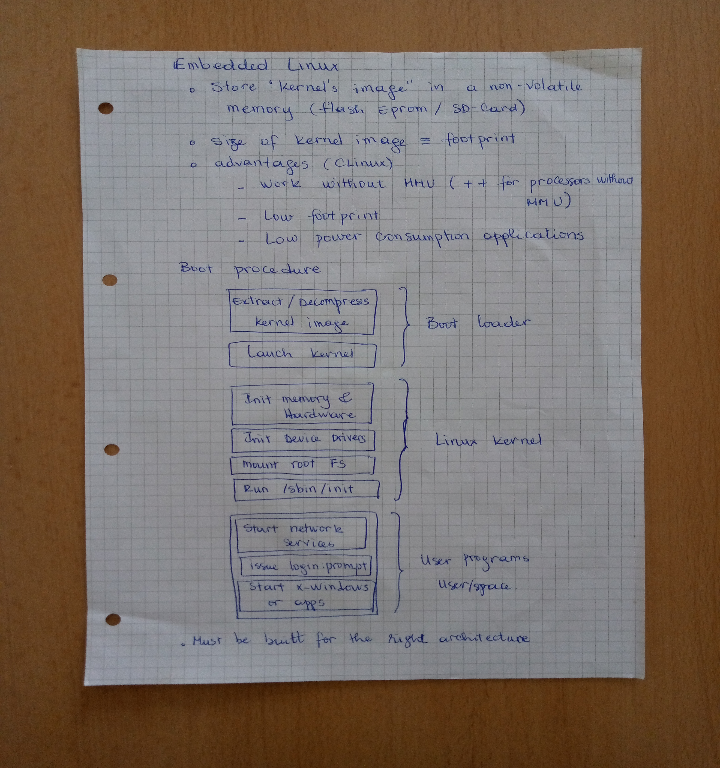
\includegraphics[width=\textwidth]{pictures/results/reference1/original.png}
      \caption{Origial image}
    \end{subfigure}
    \begin{subfigure}[b]{0.3\textwidth}
      \centering
      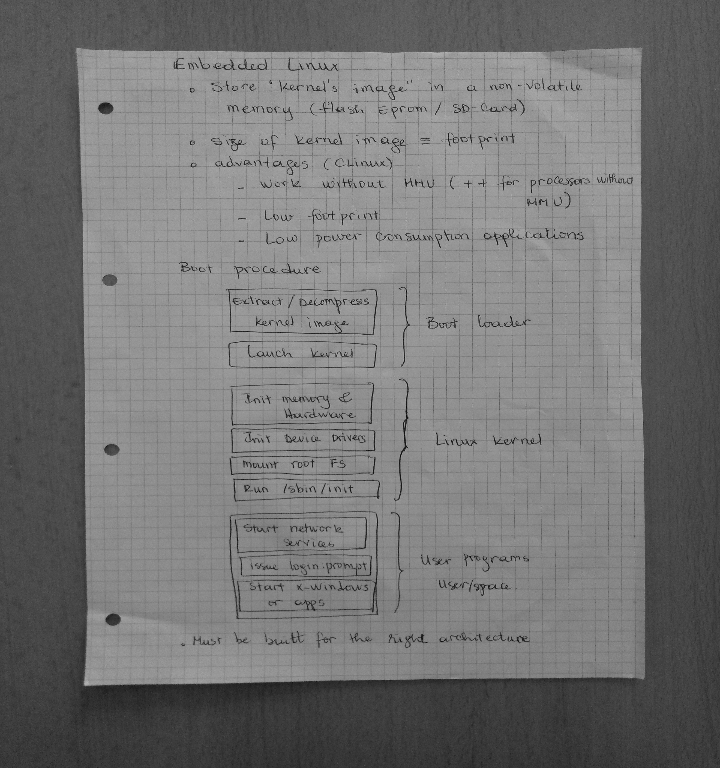
\includegraphics[width=\textwidth]{pictures/results/reference1/grayscale.png}
      \caption{Grayscale image}
    \end{subfigure}
    \begin{subfigure}[b]{0.3\textwidth}
      \centering
      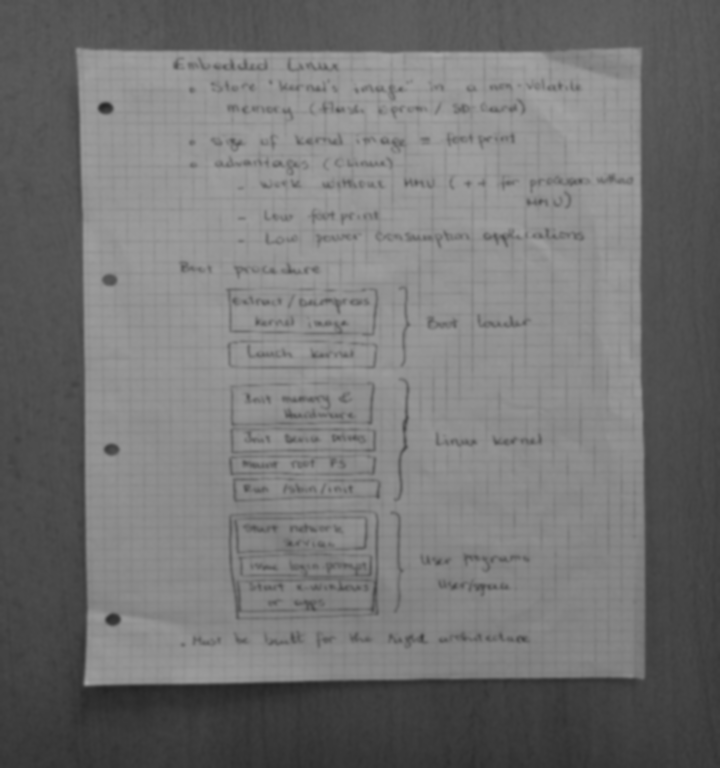
\includegraphics[width=\textwidth]{pictures/results/reference1/blur.png}
      \caption{Blured image}
    \end{subfigure}
    \vfill
    % second row
    \begin{subfigure}[b]{0.3\textwidth}
      \centering
      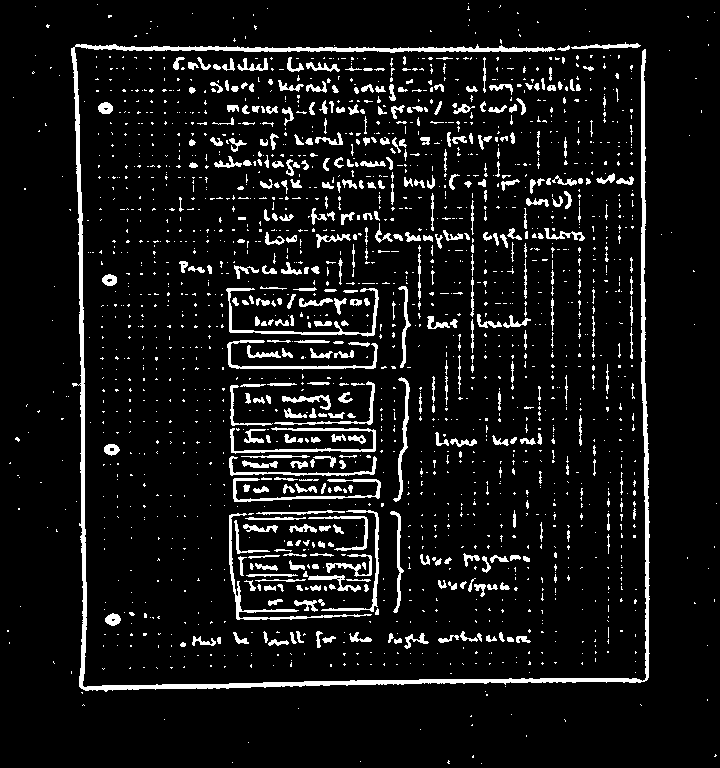
\includegraphics[width=\textwidth]{pictures/results/reference1/threshold.png}
      \caption{Thresholded image}
    \end{subfigure}
    \begin{subfigure}[b]{0.3\textwidth}
      \centering
      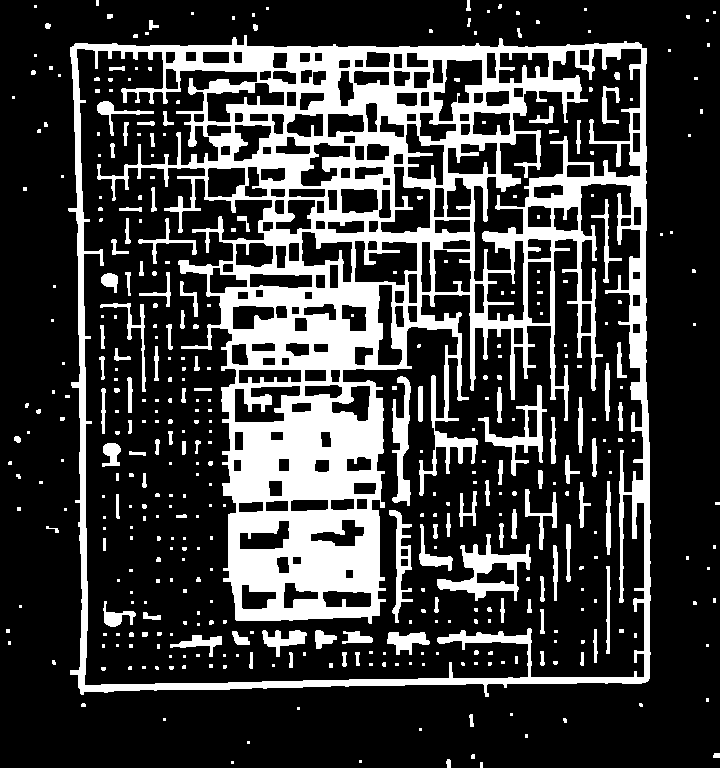
\includegraphics[width=\textwidth]{pictures/results/reference1/morphology.png}
      \caption{Morph. transformed image}
    \end{subfigure}
    \begin{subfigure}[b]{0.3\textwidth}
      \centering
      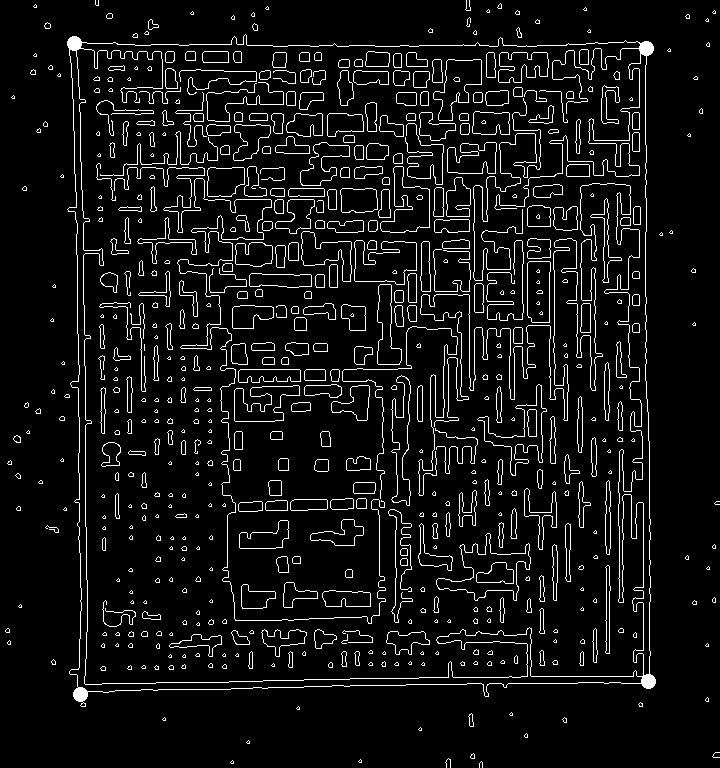
\includegraphics[width=\textwidth]{pictures/results/reference1/edge-detector.png}
      \caption{Edges \& detected corners}
    \end{subfigure}
    \vfill
    \begin{subfigure}[b]{0.3\textwidth}
      \centering
      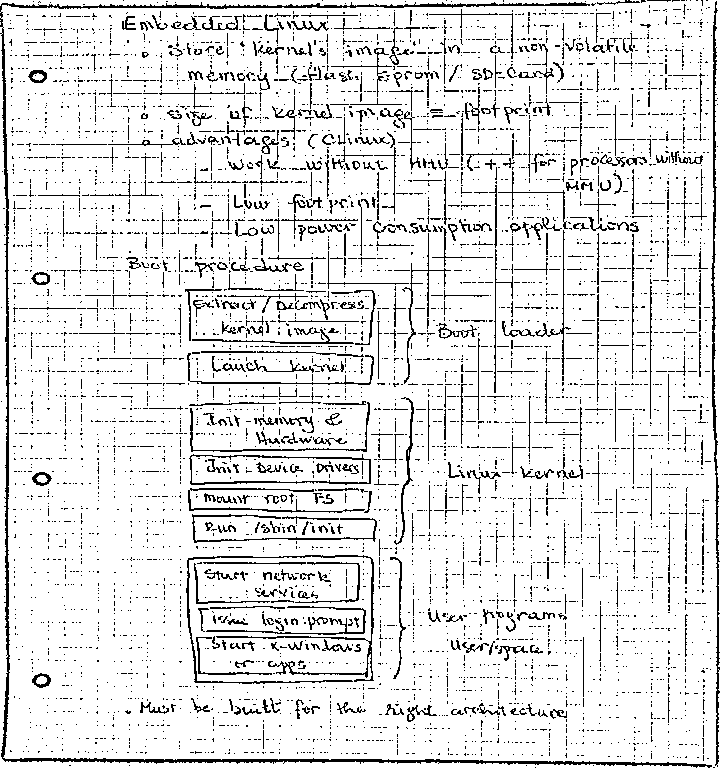
\includegraphics[width=\textwidth]{pictures/results/reference1/document.png}
      \caption{Binarized output document}
    \end{subfigure}

    \caption{Document on a table}
    \label{figure:doc-on-table}
  \end{figure}

  % Result 2
  \begin{figure}[!htbp]
    \centering
    % first row
    \begin{subfigure}[b]{0.3\textwidth}
      \centering
      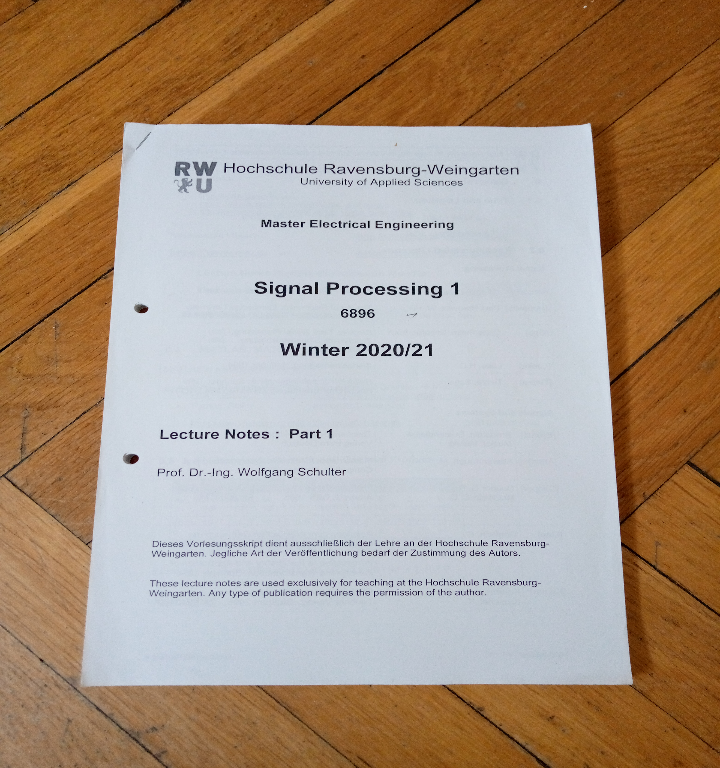
\includegraphics[width=\textwidth]{pictures/results/wood1/original.png}
      \caption{Origial image}
    \end{subfigure}
    \begin{subfigure}[b]{0.3\textwidth}
      \centering
      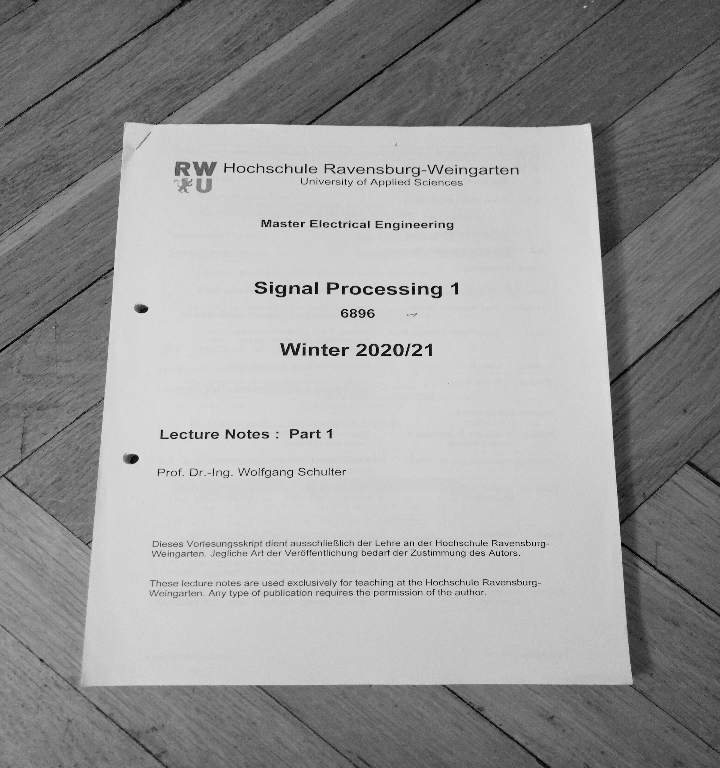
\includegraphics[width=\textwidth]{pictures/results/wood1/grayscale.png}
      \caption{Grayscale image}
    \end{subfigure}
    \begin{subfigure}[b]{0.3\textwidth}
      \centering
      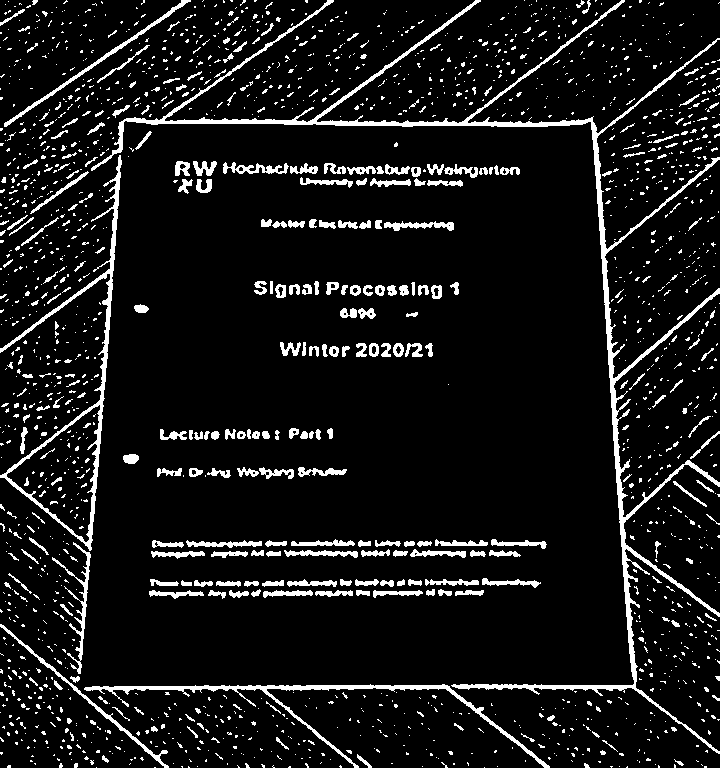
\includegraphics[width=\textwidth]{pictures/results/wood1/threshold.png}
      \caption{Thresholded image}
    \end{subfigure}
    \vfill
    % second row
    \begin{subfigure}[b]{0.3\textwidth}
      \centering
      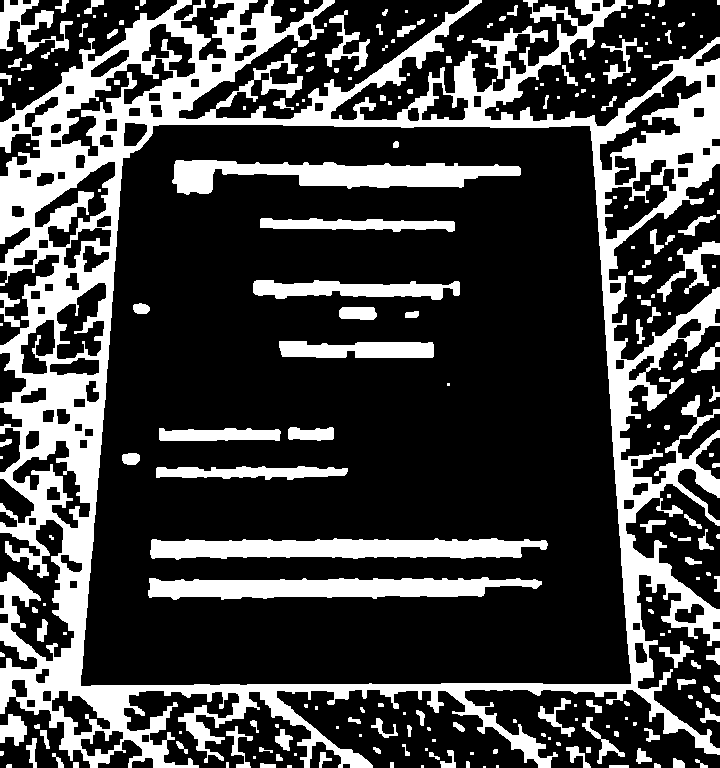
\includegraphics[width=\textwidth]{pictures/results/wood1/morphology.png}
      \caption{Morph. transformed image}
    \end{subfigure}
    \begin{subfigure}[b]{0.3\textwidth}
      \centering
      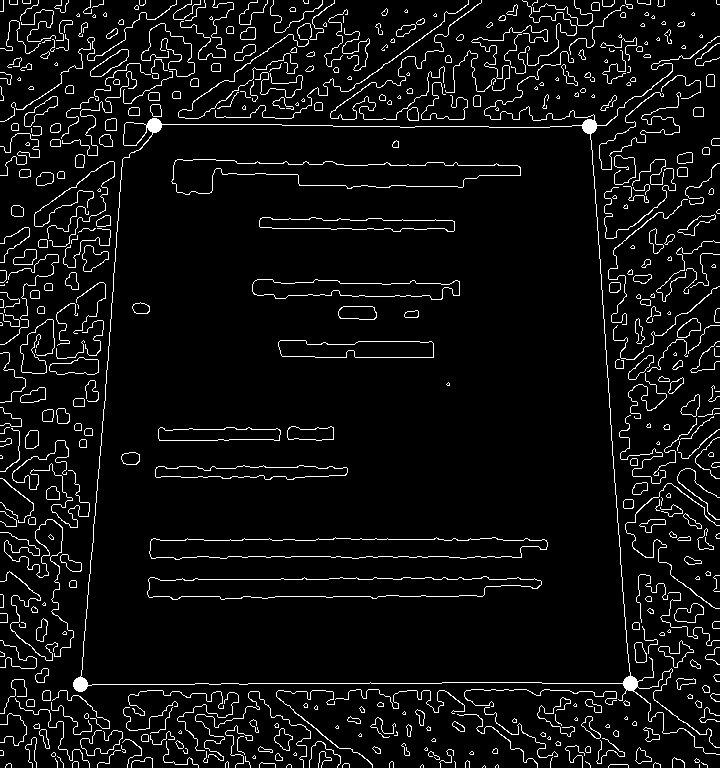
\includegraphics[width=\textwidth]{pictures/results/wood1/edge-detector.png}
      \caption{Edges \& detected corners}
    \end{subfigure}
    \begin{subfigure}[b]{0.3\textwidth}
      \centering
      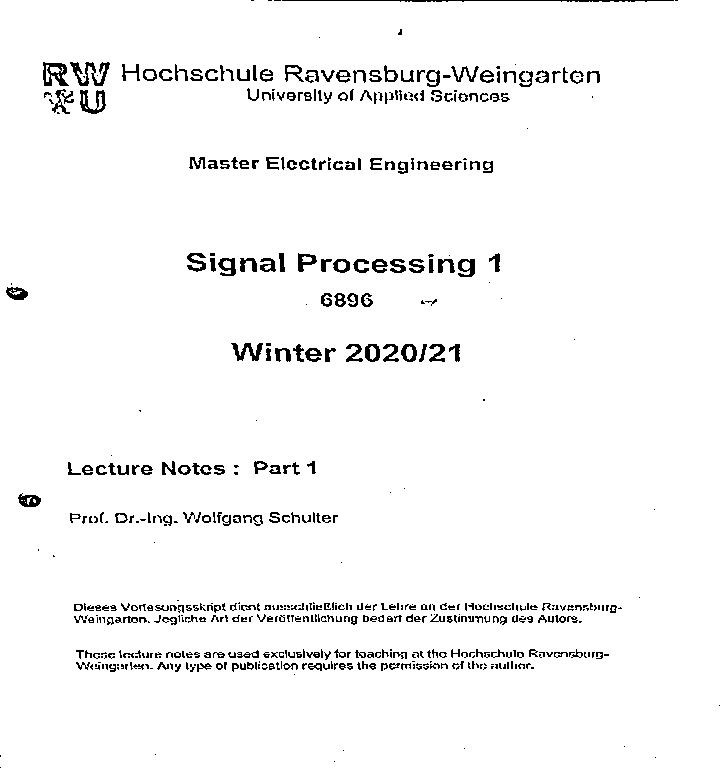
\includegraphics[width=\textwidth]{pictures/results/wood1/document.png}
      \caption{Binarized output document}
    \end{subfigure}

    \caption{Document on a wooden floor}
    \label{figure:doc-on-wooden-floor}
  \end{figure}

  % Result 3
  \begin{figure}[!htbp]
    \centering
    % first row
    \begin{subfigure}[b]{0.3\textwidth}
      \centering
      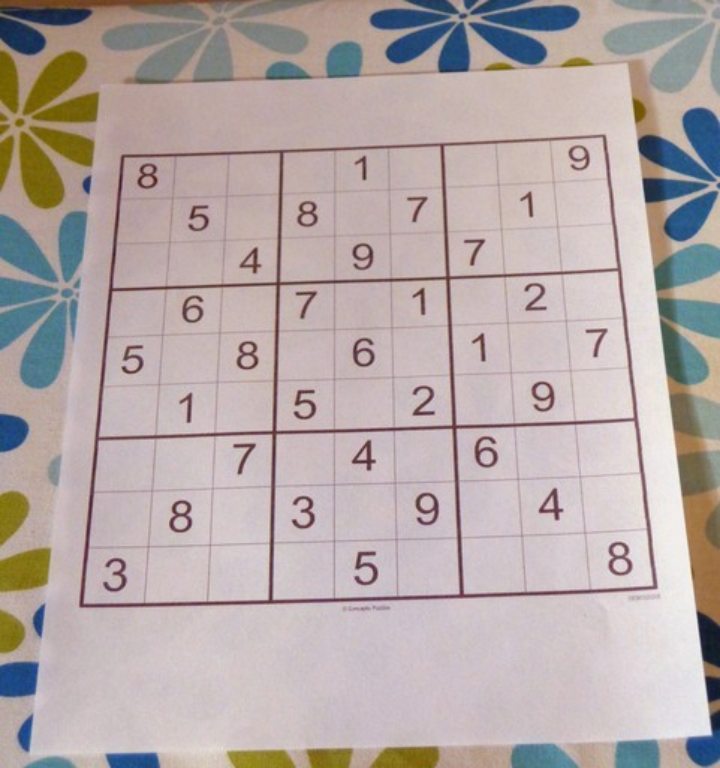
\includegraphics[width=\textwidth]{pictures/results/sudoku/original.png}
      \caption{Origial image}
    \end{subfigure}
    \begin{subfigure}[b]{0.3\textwidth}
      \centering
      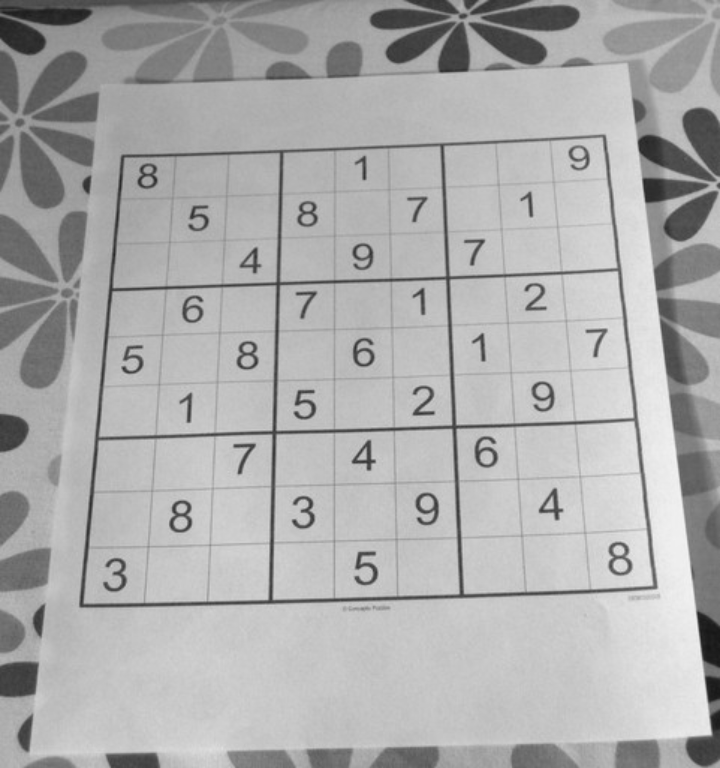
\includegraphics[width=\textwidth]{pictures/results/sudoku/grayscale.png}
      \caption{Grayscale image}
    \end{subfigure}
    \begin{subfigure}[b]{0.3\textwidth}
      \centering
      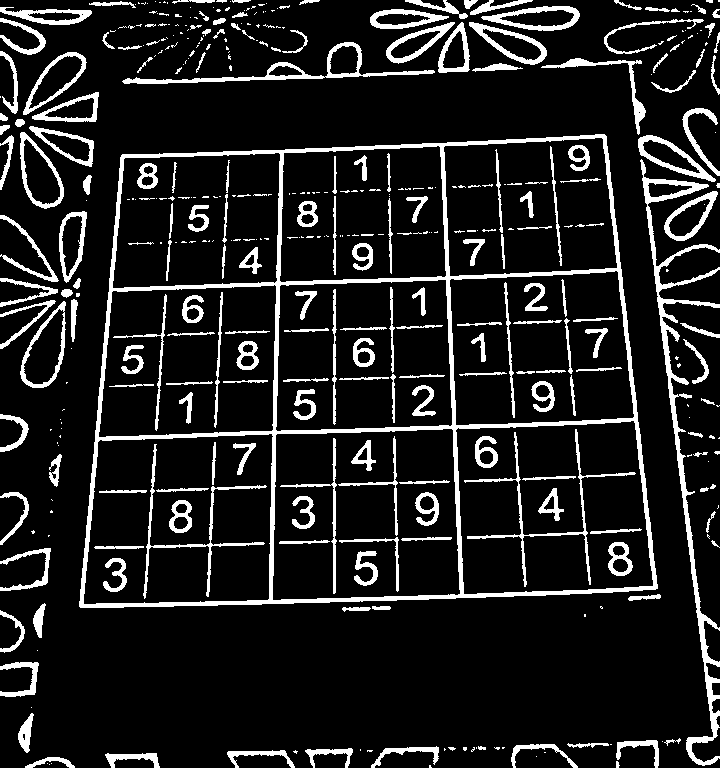
\includegraphics[width=\textwidth]{pictures/results/sudoku/threshold.png}
      \caption{Thresholded image}
    \end{subfigure}
    \vfill
    % second row
    \begin{subfigure}[b]{0.3\textwidth}
      \centering
      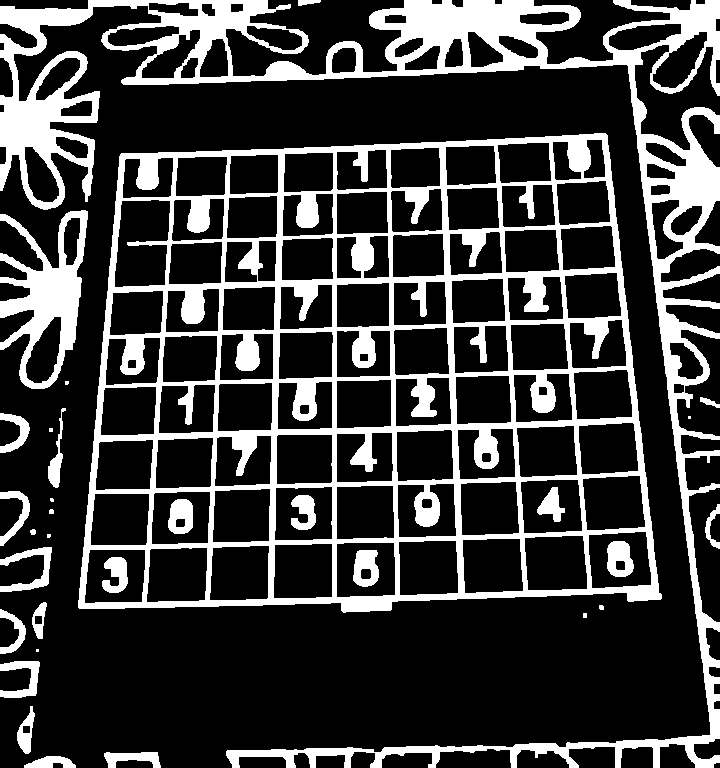
\includegraphics[width=\textwidth]{pictures/results/sudoku/morphology.png}
      \caption{Morph. transformed image}
    \end{subfigure}
    \begin{subfigure}[b]{0.3\textwidth}
      \centering
      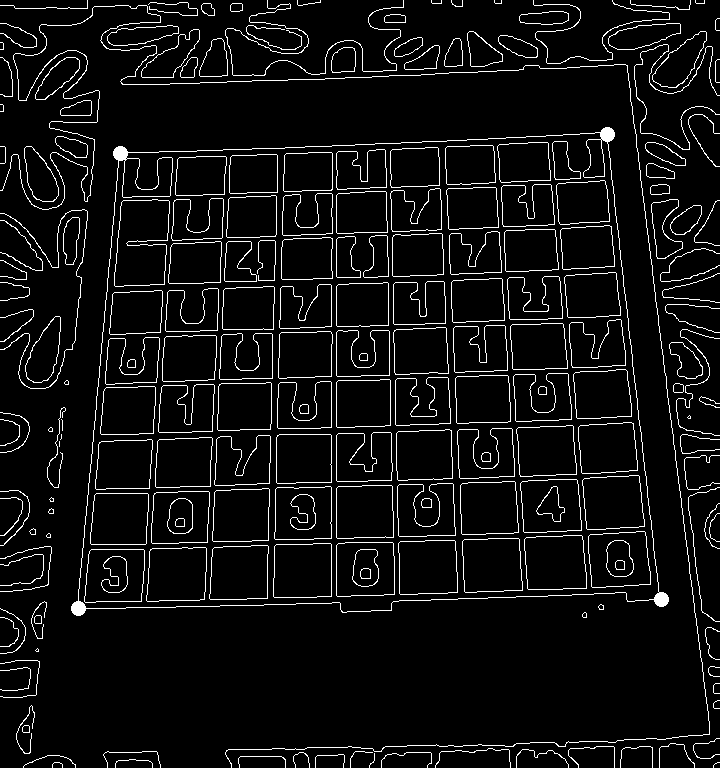
\includegraphics[width=\textwidth]{pictures/results/sudoku/edge-detector.png}
      \caption{Edges \& detected corners}
      \label{figure:doc-on-table-patterns--edges}
    \end{subfigure}
    \begin{subfigure}[b]{0.3\textwidth}
      \centering
      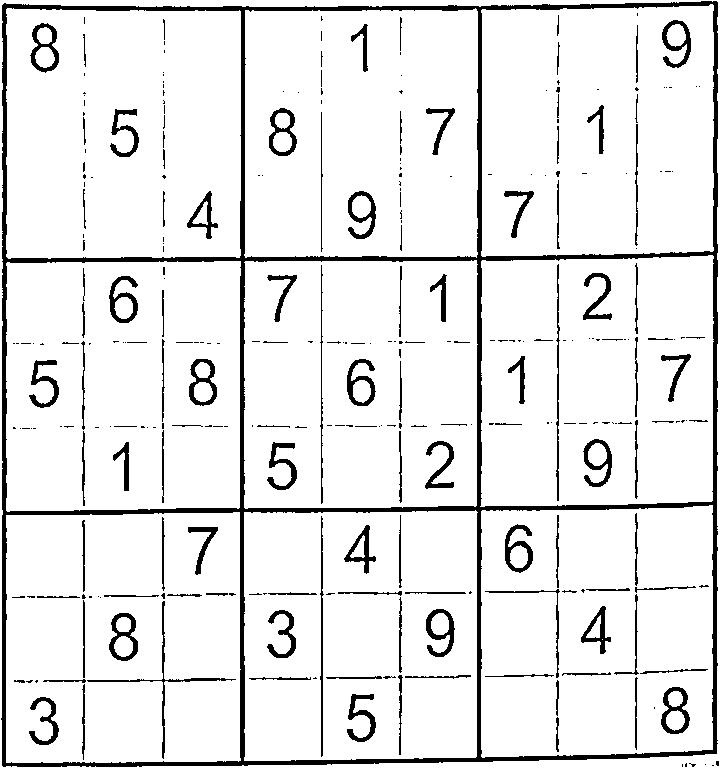
\includegraphics[width=\textwidth]{pictures/results/sudoku/document.png}
      \caption{Binarized output document}
    \end{subfigure}

    \caption{Document on a background with patterns}
    \label{figure:doc-on-table-patterns}
  \end{figure}

  % Result 4
  \begin{figure}[!htbp]
    \centering
    % first row
    \begin{subfigure}[b]{0.3\textwidth}
      \centering
      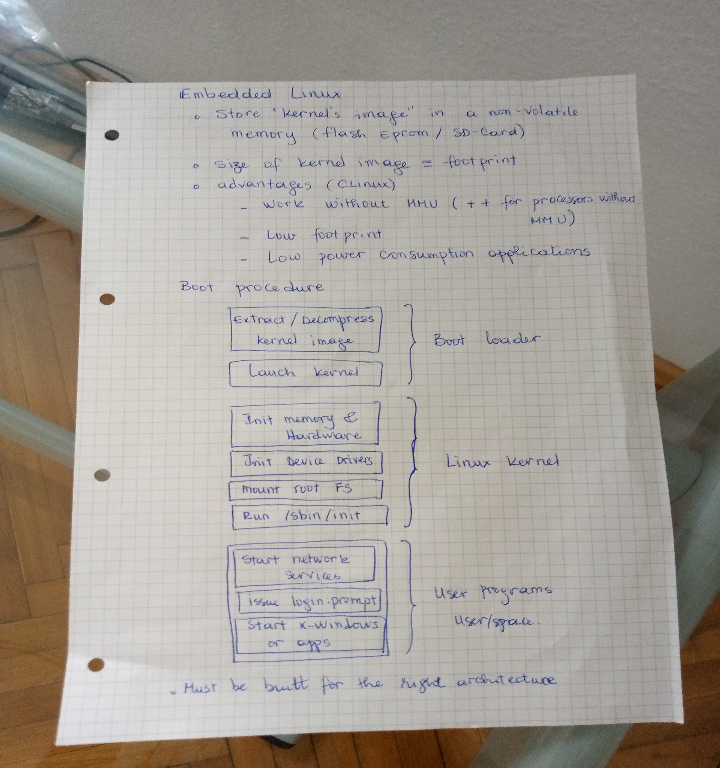
\includegraphics[width=\textwidth]{pictures/results/glass/original.png}
      \caption{Origial image}
    \end{subfigure}
    \begin{subfigure}[b]{0.3\textwidth}
      \centering
      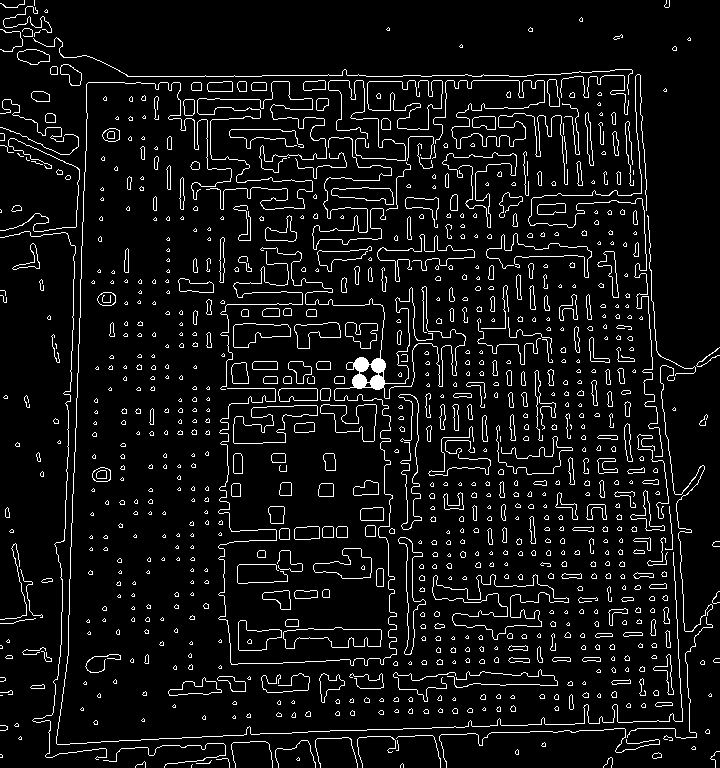
\includegraphics[width=\textwidth]{pictures/results/glass/edge-detector.png}
      \caption{Edges \& detected corners}
    \end{subfigure}
    \caption{Document on a glass table}
    \label{figure:document-on-glass-table}
  \end{figure}

  % Result 5
  \begin{figure}[!htbp]
    \centering
    % first row
    \begin{subfigure}[b]{0.3\textwidth}
      \centering
      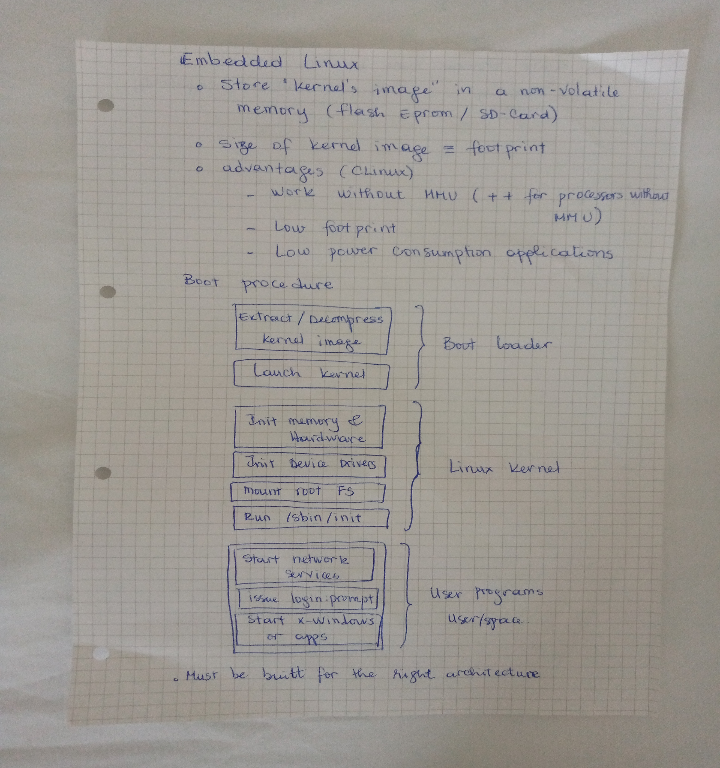
\includegraphics[width=\textwidth]{pictures/results/white1/original.png}
      \caption{Origial image}
    \end{subfigure}
    \begin{subfigure}[b]{0.3\textwidth}
      \centering
      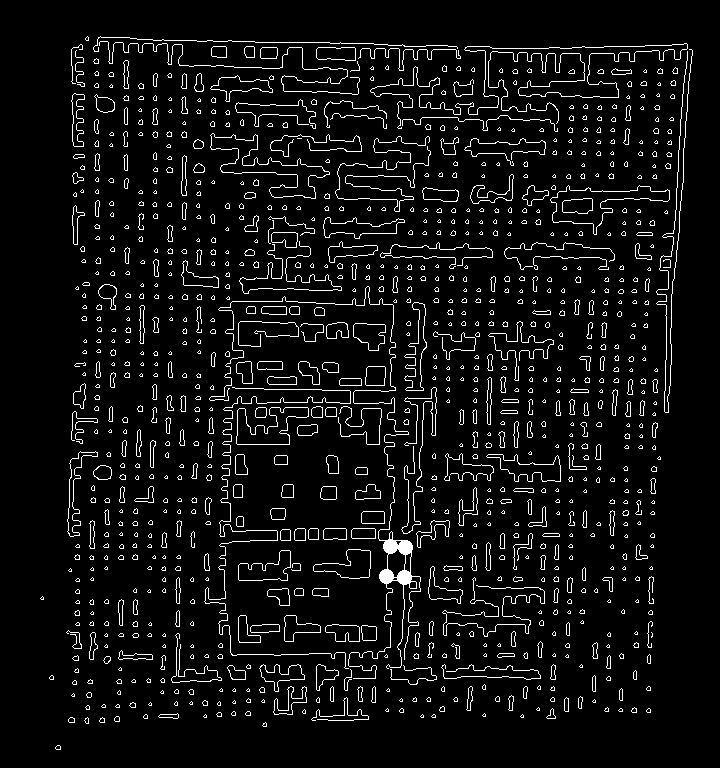
\includegraphics[width=\textwidth]{pictures/results/white1/edge-detector.png}
      \caption{Edges \& detected corners}
    \end{subfigure}
    \caption{Book on a white background}
    \label{figure:document-on-white-background}
  \end{figure}

  % Result 6
  \begin{figure}[!htbp]
    \centering
    % first row
    \begin{subfigure}[b]{0.3\textwidth}
      \centering
      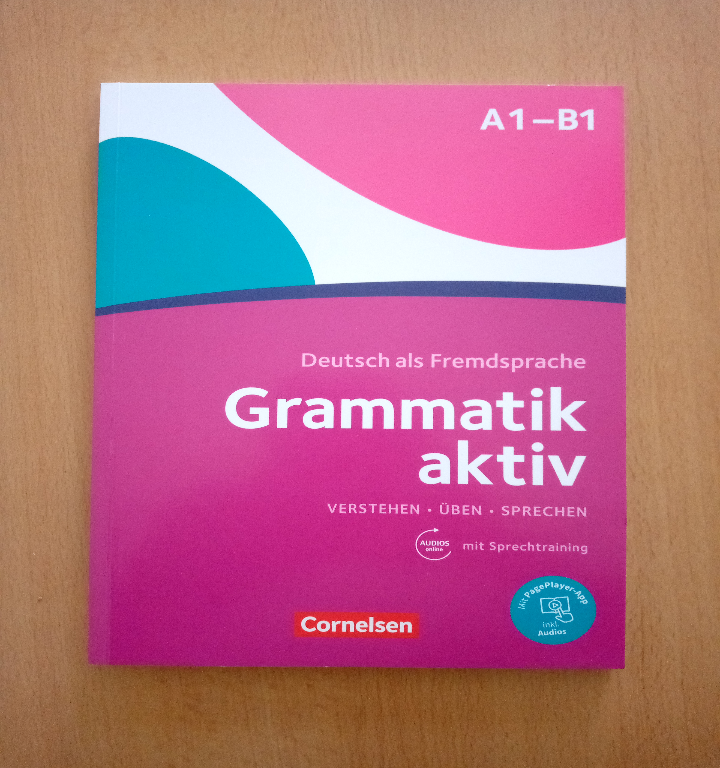
\includegraphics[width=\textwidth]{pictures/results/reference4/original.png}
      \caption{Origial image}
    \end{subfigure}
    \begin{subfigure}[b]{0.3\textwidth}
      \centering
      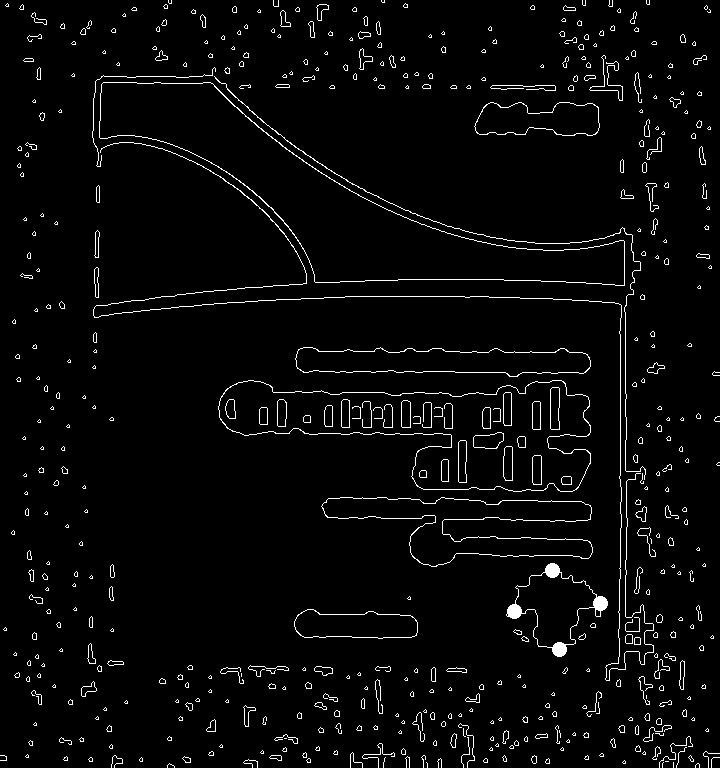
\includegraphics[width=\textwidth]{pictures/results/reference4/edge-detector.png}
      \caption{Edges \& detected corners}
    \end{subfigure}
    \caption{Book on a table}
    \label{figure:book-on-table}
  \end{figure}

  \section{Conclusion}

  In order to achieve the document scanner, two pipelines have been implemented. The first
  for detecting and getting the corners of the document and the second for extracting the
  document from the image and performing its binarization. Although the proposed pipeline
  worked for some images, it still fails on others for different reasons (lighting,
  background, etc.).

  The order of the pipelines' stages and the different paramaters required for each of them 
  actually define how the pipelines behaves. Therefore the difficulty of the task resides
  in finding the correct order for the different stages as well as the right value of the
  paramaters.

  The corner detection is based on detecting the contour of the document and finding an
  approximated rectangle around it. So a failure in the contour detection prevent from getting
  a scanned document. As so, another method that can the used is
  \textit{Hough line transformation} \cite{cv-img-hough-transform}.

  However, that does not change the fact that there is still so many possibility for designing
  a pipeline for scanning a document. So, it's more interresting to find an optimal solution
  to automatically find the right order and the right parameters. That solution would be
  \textit{Deep learning}. Therefore, a recommended method for further work would be to
  gather enough dataset of pictures of documents, label them (marking the corners) and
  train a neural network for document's corner detection.

  \printbibliography
\end{document}
